\documentclass[mathserif,handout]{beamer} % Math 298 Fall 2014
%\usepackage{mybeamertheme}
\usepackage{pdfsync} % works only on TeXShop, comment otherwise
\usepackage{pgf}
\usepackage{multimedia} % to embed movies in the PDF file
\usepackage{xcolor}
\usepackage{graphicx}
\usepackage{comment}
\usepackage{pgfpages}
\usepackage{topcapt}
\usepackage{booktabs}

% for the tikz pictures
\usepackage{geometry}
%\geometry{hmargin=1cm,vmargin=1cm}
\usepackage{tikz}
\def\width{5}
\def\hauteur{5}

\mode<presentation>
{
  \usetheme{Madrid}   %  \usetheme{Warsaw}
  % Note: this next command makes nice slides, but Adobe doesn't like it (you get blank pages)
  \setbeamertemplate{background canvas}[vertical shading][bottom=white,top=structure.fg!15]
  %\setbeamertemplate{footline}{\pgfuseimage{UCM-logo}}

  %\usecolortheme{seahorse}
  \usecolortheme{beaver}
 % \setbeamercovered{transparent}
}
%\usepackage[T1]{fontenc}
% For printing purposes only
%\pgfpagesuselayout{4 on 1}[letterpaper,border shrink=5mm,landscape]  % print out 4 slides to a page
\pgfpagesuselayout{resize to}[letterpaper,border shrink=5mm,landscape]  % print out full size on paper
  
\usepackage{amssymb,amsmath}
\hypersetup{%
 pdftitle={Math298 Lecture 4},
 pdfauthor={Juan Meza(UC Merced)},
 pdfsubject={Fundamental Concepts in Computational and Applied Mathematics},
 pdfkeywords={linear algebra, sparse, structured grids}
 }
 
\title[Math 298 Lecture 5b]{Fundamental Concepts in \\ Computational and Applied Mathematics}  \subtitle{}
\author[Juan Meza]{Juan Meza \\ School of Natural Sciences \\ University of California, Merced}
\date[Fall 2014]{Fall 2014}
\institute[UC Merced]

\pgfdeclareimage[width=\textwidth]{CFLcondition}{CFLcondition}

% \logo{\pgfuseimage{UCM-logo}}

%% figures






% Common abbreviations
% (Remember to put '\ ' after if an interword space is
%  desired rather than end-of-sentence space. Same for '.etc)' ).
\newcommand{\eg}{{\em e.g.}}		% e.g.
\newcommand{\ie}{{\em i.e.}}		% i.e.
\newcommand{\etc}{{\em etc.}}		% etc.
\newcommand{\vs}{{\em vs.}}		% vs.
\newcommand{\remark}{{\color{red} Remark:} }


\newcommand {\DS} {\displaystyle}
\newcommand{\eref}[1]{{\rm{(\ref{#1})}}}
\newcommand{\tref}[1]{{\rm{\ref{#1}}}}


\def\frechet{Fr\'echet\ }
\def\more{Mor\'e\ }
\def\fl{{\sf fl}}
\def\flop{{\sf flop} }
\def\flops{{\sf flops} }
\def\matlab{{\sc Matlab} }
\def\Matlab{\matlab}

\def\bigO{\mathcal{O}}

% Mathematical Symbols

\newcommand{\deq}{\raisebox{0pt}[1ex][0pt]{$\stackrel{\scriptscriptstyle{\rm def}}{{}={}}$}}

\newcommand {\half} {\mbox{$\frac{1}{2}$}}  %machine epsilon
\newcommand{\set}[2]{\left\{ #1 \;:\; #2 \right\}}

\newcommand {\macheps} {\mathbf{\epsilon}}  %machine epsilon
\newcommand {\real} {\mathbb{R}}
\newcommand {\nat} {\mathbb{N}}
\newcommand {\compl} {\mathbb{C}}
\newcommand {\diag} {{\mbox{diag}}}
\newcommand {\meas} {{\mbox{meas}}}
\newcommand {\mspan} {{\mbox{span}}}

\newcommand {\pdx} {\frac{\partial}{\partial x}}
\newcommand {\pdt} {\frac{\partial}{\partial t}}
\newcommand {\pdxx} {\frac{\partial^2}{\partial x^2}}
\newcommand {\dx} {\frac{d}{d x}}
\newcommand {\dt} {\frac{d}{d t}}
\newcommand {\dxx} {\frac{d^2}{d x^2}}

\newcommand {\bA} {\mbox{\boldmath $A$}}
\newcommand {\bB} {\mbox{\boldmath $B$}}
\newcommand {\bF} {\mbox{\boldmath $F$}}
\newcommand {\bI} {\mbox{\boldmath $I$}}
\newcommand {\bP} {\mbox{\boldmath $P$}}
\newcommand {\bY} {\mbox{\boldmath $Y$}}
\newcommand {\bZ} {\mbox{\boldmath $Z$}}
\newcommand {\ba} {\mbox{\boldmath $a$}}
\newcommand {\bb} {\mbox{\boldmath $b$}}
\newcommand {\bd} {\mbox{\boldmath $d$}}
\newcommand {\bff}{\mbox{\boldmath $f$}}
\newcommand {\bk} {\mbox{\boldmath $k$}}
\newcommand {\bp} {\mbox{\boldmath $p$}}
\newcommand {\bs} {\mbox{\boldmath $s$}}
\newcommand {\bu} {\mbox{\boldmath $u$}}
\newcommand {\bv} {\mbox{\boldmath $v$}}
\newcommand {\bw} {\mbox{\boldmath $w$}}
\newcommand {\bx} {\mbox{\boldmath $x$}}
\newcommand {\by} {\mbox{\boldmath $y$}}
\newcommand {\bz} {\mbox{\boldmath $z$}}
\newcommand {\blambda} {\mbox{\boldmath $\lambda$}}
\newcommand {\btau} {\mbox{\boldmath $\tau$}}

%
% JCM Quantum Chemistry commands
%
\newcommand{\bra}[1]{\langle #1|}
\newcommand{\ket}[1]{|#1\rangle}
\newcommand{\braket}[2]{\langle #1|#2\rangle}
% Example of usage
%\[
%\ket{\Psi}=\sum_{i}\ket{\phi_i}\braket{\phi_i}{\Psi}
%\]

%
% Other symbols
%
\newcommand {\grad}{\nabla}
\newcommand {\hess}{\nabla^2}
\newcommand {\condA}{\kappa(A)}

\newtheorem{algorithm}{Algorithm}

%

% \boxfig{pos}{wid}{text}:  A figure with a box around it
%
% pos	the usual figure placement arg: eg. htbp
% wid	the width of the figure, in some units: eg. 5in
% text	the contents of the figure, including picture/caption/label/etc
%
\newlength{\boxwidth}
\newcommand{\boxfigure}[3]{
	\begin{figure}[#1]
		\setlength{\boxwidth}{#2}
		\addtolength{\boxwidth}{.1in}

		\centering
		\framebox[\boxwidth]{
			\begin{minipage}{#2}
			#3
			\end{minipage}
		}
	\end{figure}  
}

% use \fullboxwidth for arg 2 of boxfigure to get box of size \textwidth


% \boxalg{pos}{text}:  An algorithm with a box around it
%
% title  the name of the algorithm
% text   the contents of the figure, including picture/caption/label/etc
%
\newcommand{\boxalg}[2]{
            \setlength{\boxwidth}{\fullboxwidth}
            \addtolength{\boxwidth}{.1in}
            \vspace{2ex}
            \framebox[\boxwidth][#1]{
                    \vspace{1ex}
                    \begin{minipage}{\fullinboxwidth}
                        #2
                    \end{minipage}
                    \vspace{1ex}
            }
            \vspace{2ex}
}






% see above
\newlength{\fullboxwidth}
\setlength{\fullboxwidth}{\textwidth}
\addtolength{\fullboxwidth}{-0.5in}

\newlength{\fullinboxwidth}
\setlength{\fullinboxwidth}{\fullboxwidth}
\addtolength{\fullinboxwidth}{-0.5in}






\definecolor{navy}{RGB}{0,0,128}
\definecolor{forestgreen}{RGB}{34,139,34}
\definecolor{mylightsteelblue}{RGB}{176,196,222}
\definecolor{mylightcyan}{RGB}{180,255,255}
\definecolor{mypaleturquoise}{RGB}{175,238,238}
\definecolor{mylightgoldenrod}{RGB}{250,250,210}
\definecolor{mylightyellow}{RGB}{255,255,224}
\definecolor{mylightsalmon}{RGB}{255,160,122}

\setbeamercolor{blacklightsteelblue}{fg=black,bg=mylightsteelblue}
\setbeamercolor{blackpaleturquoise}{fg=black,bg=mypaleturquoise}
\setbeamercolor{blacklightcyan}{fg=black,bg=mylightcyan}
\setbeamercolor{blacklightgoldenrod}{fg=black,bg=mylightgoldenrod}
\setbeamercolor{blacklightyellow}{fg=black,bg=mylightyellow}
\setbeamercolor{blacklightsalmon}{fg=black,bg=mylightsalmon}
\setbeamercolor{blackcyan}{fg=black,bg=cyan}




\begin{document}

%%%%%%%%%%%%%%%%%%%%%%%%%%%%%%%%%%%%%%%%%%%%%
\frame{
\titlepage
} % end frame

\section{Introduction}
%%%%%%%%%%%%%%%%%%%%%%%%%%%%%%%%%%%%%%%%%%%%%
\frame{\frametitle{Introduction}
\begin{itemize}
\item Elementary discussion of algebraic problems arising in discretization of differential equations
\item Behavior of the solution as mesh width tends to zero
\item Treat BVP end EV problems for elliptic pdes and IVP for hyperbolic and parabolic pdes 

\item For elliptic
\end{itemize}
} % end frame

%%%%%%%%%%%%%%%%%%%%%%%%%%%%%%%%%%%%%%%%%%%%%
\frame{\frametitle{Main Results}
\begin{itemize}
\item For elliptic equations a difference quotient tends to the corresponding derivative
\item For elliptic equations convergence is guaranteed independently of mesh
\item For hyperbolic equations convergence is obtained iff certain ratio of mesh width is satisfied 
\end{itemize}
} % end frame

%%%%%%%%%%%%%%%%%%%%%%%%%%%%%%%%%%%%%%%%%%%%%
\frame{\frametitle{Outline}
\begin{itemize}
\item Introduction
\item Elliptic equations 
\item Hyperbolic equations
\end{itemize}
} % end frame

%%%%%%%%%%%%%%%%%%%%%%%%%%%%%%%%%%%%%%%%%%%%%
\frame{\frametitle{Motivation}

\begin{itemize}
\item Consider case in 1D, on an equally spaced grid $u(x)$
\item $h$ is the spatial discretization

\vspace{.25in}

\end{itemize}
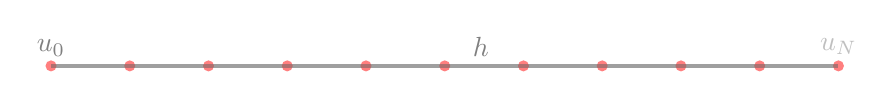
\begin{tikzpicture}[x=1cm, y=1cm, semitransparent]
%\draw[step=1mm, line width=0.1mm, black!30!white] (0,0) grid (\width,\hauteur);
%\draw[step=5mm, line width=0.2mm, black!40!white] (0,0) grid (\width,\hauteur);
\draw[step=5cm, line width=0.5mm, black!50!white] (0,0) grid (10,0);
%\draw[step=1cm, line width=0.5mm, black!50!white] (1,1) grid (10,0);


    \coordinate (u0) at (0,0)     node[above]  {$u_0$};  
    \coordinate (u1) at (1,0);
    \coordinate (u2) at (2,0);
    \coordinate (u3) at (3,0);
    \coordinate (u4) at (4,0);
    \coordinate (u5) at (5,0);
    \coordinate (u6) at (6,0);
    \coordinate (u7) at (7,0);
    \coordinate (u8) at (8,0);
    \coordinate (u9) at (9,0);
    \coordinate (u10) at (10,0);
    \fill[red] (u0) circle (2pt);
    \fill[red] (u1) circle (2pt);
    \fill[red] (u2) circle (2pt);
    \fill[red] (u3) circle (2pt);
    \fill[red] (u4) circle (2pt);
     \fill[red] (u5) circle (2pt) node[ above right ] {$\ \ {\color{black} h}$};
     \fill[red] (u6) circle (2pt);
     \fill[red] (u7) circle (2pt);
     \fill[red] (u8) circle (2pt);    
     \fill[red] (u9) circle (2pt);
     \fill[red] (u10) circle (2pt);

\draw[step=1cm, line width=0.5mm, black!50!white] (0,0) grid (10,0)     node[above] {$u_N$};;

                
\end{tikzpicture}
$$
u_{x} = \frac{u(x_{j+1}) - u(x_{j-1})}{2h}
$$
} % end frame

%%%%%%%%%%%%%%%%%%%%%%%%%%%%%%%%%%%%%%%%%%%%%
\frame{\frametitle{Likewise in 2D}

\begin{columns}[c]
\begin{column}{.4\textwidth}
\begin{eqnarray*}
u_{x} &=& \frac{u(x+h,y) - u(x,y)}{h} \\
u_{y} &=& \frac{u(x,y+h) - u(x,y)}{h} \\
u_{\bar{x}} &=& \frac{u(x,y) - u(x - h,y)}{h} \\
u_{\bar{y}} &=& \frac{u(x,y) - u(x, y-h)}{h} 
\end{eqnarray*}

\end{column}

\begin{column}{.6\textwidth}
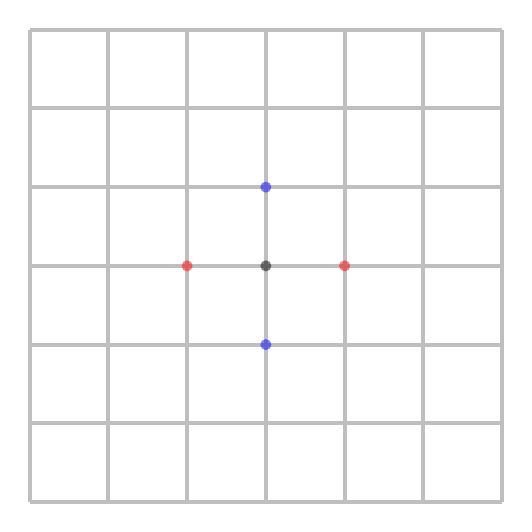
\begin{tikzpicture}[x=1cm, y=1cm, semitransparent]
%\draw[step=1mm, line width=0.1mm, black!30!white] (0,0) grid (\width,\hauteur);
%\draw[step=5mm, line width=0.2mm, black!40!white] (0,0) grid (\width,\hauteur);
%\draw[step=5cm, line width=0.5mm, black!50!white] (0,0) grid (\width,\hauteur);
\draw[step=1cm, line width=0.5mm, black!50!white] (-1,-1) grid (\width,\hauteur);
    \coordinate (u0) at (2,2);
    \coordinate (u1) at (2,1);
    \coordinate (u2) at (1,2);
    \coordinate (u3) at (3,2);
    \coordinate (u4) at (2,3);
    \fill[black] (u0) circle (2pt);
    \fill[blue] (u1) circle (2pt);
    \fill[red] (u2) circle (2pt);
    \fill[red] (u3) circle (2pt);
    \fill[blue] (u4) circle (2pt);
\end{tikzpicture}
\end{column}
\end{columns}
$$u_{xx} = \frac{u(x+h,y) - 2u(x,y) + u(x-h,y)}{h}$$
} % end frame


%%%%%%%%%%%%%%%%%%%%%%%%%%%%%%%%%%%%%%%%%%%%%
\frame{\frametitle{Definitions}
\begin{itemize}
\item Introduction
\item Elliptic equations: $$ \frac{\partial^2 u}{\partial t^2} + \frac{\partial^2 u}{\partial x^2} = 0 $$ or $$ \Delta u = u_{xx} + u_{yy}$$
\item Hyperbolic equations: $$ \frac{\partial^2 u}{\partial t^2} - \frac{\partial^2 u}{\partial x^2} = 0 $$
\end{itemize}
} % end frame

%%%%%%%%%%%%%%%%%%%%%%%%%%%%%%%%%%%%%%%%%%%%%
\frame{\frametitle{Main Results: Section 1}

Assume 
\begin{itemize}
\item a simply connected region $G$ with boundary $\partial G$, 
\item $f(x,y)$ is a given continuous function 
\item $f(x,y)$ has continuous first and second partial derivatives in a region containing $G$.
\item a mesh $G_h$, with mesh width $h$,
\item $u_h(x,y)$ is the solution of the difference equation $\Delta u = 0$. 
\end{itemize}

Then 
\begin{itemize}
\item As $h \rightarrow 0$, $u_h (x,y)$ converges to $u(x,y)$ satisfying the pde on the domain $G$ and equals $f$ on the boundary 
\item For any interior region within $G$ the difference quotients, $u_h$ tend to the corresponding partial derivatives of $u(x,y)$
\end{itemize}
} % end frame

%%%%%%%%%%%%%%%%%%%%%%%%%%%%%%%%%%%%%%%%%%%%%
\frame{\frametitle{Main Results: Section 2}
Assume 
\begin{itemize}
\item Hyperbolic equation: $$ \frac{\partial^2 u}{\partial t^2} - \frac{\partial^2 u}{\partial x^2} = 0 $$
\item a rectangular mesh, with mesh size $h$ in the time direction, and $kh$, in the spatial ($x$) direction
\end{itemize}

\begin{itemize}
\item For $k < 1$, as $h \rightarrow 0$, the solution to the difference equation cannot converge to the solution of the differential equation
\end{itemize}

In other words for:
$$
k = \frac{\Delta x}{\Delta t} < 1 
$$
the difference quotient solution will not converge!!!
} % end frame

%%%%%%%%%%%%%%%%%%%%%%%%%%%%%%%%%%%%%%%%%%%%%
\frame{\frametitle{Main Results: CFL Condition Pictorially \footnote {{\scriptsize Content under Creative Commons Attribution license CC-BY 4.0, code under MIT license (c)2014 L.A. Barba, G.F. Forsyth, C. Cooper. Based on CFDPython, (c)2013 L.A. Barba, also under CC-BY license.}}}

	\pgfputat{\pgfxy(0.0,-3.0)}{\pgfbox[left,base]{\pgfuseimage{CFLcondition}}}
	

} % end frame


%%%%%%%%%%%%%%%%%%%%%%%%%%%%%%%%%%%%%%%%%%%%%
\frame{\frametitle{Main Results: CFL Condition}

Today for the general wave equation with velocity $c$: 

$$ \frac{\partial^2 u}{\partial t^2} - c \frac{\partial^2 u}{\partial x^2} = 0, $$

we say that the time step $\Delta t$ must be chosen so that the CFL condition is met, i.e.:
$$
\sigma = c \frac{\Delta t}{\Delta x} \leq \sigma_{max} 
$$
\begin{block}{Note:}
The value of $\sigma_{max}$ will vary according to the numerical method used.  For an explicit method, $\sigma_{max}$ is typically 1.
\end{block}
} % end frame


%%%%%%%%%%%%%%%%%%%%%%%%%%%%%%%%%%%%%%%%%%%%%
\begin{frame}[allowframebreaks]
  \frametitle<presentation>{References}    
  \begin{thebibliography}{10}    
  \beamertemplateonlinebibitems
 \bibitem{Bakker2002}
   Andre Bakker.
    \newblock {\em Lecture 7 - Meshing}.
   \newblock http://www.bakker.org/dartmouth06/engs150/07-mesh.pdf
  \beamertemplatebookbibitems
 \bibitem{Iserles09}
   Arieh Iserles.
    \newblock {\em A First Course in the Numerical Analysis of Differential Equations, 2nd Ed.},
   \newblock Cambridge University Press, 2009.
     \beamertemplatearticlebibitems
 \bibitem{CFL}
 R. Courant, K. Friedrichs, H. Lewy.
  \newblock On the Partial Difference Equations of Mathematical Physics,
 \newblock IBM Journal, March 1967.
 \end{thebibliography}

\end{frame}% end frame

\end{document}
